\documentclass[border=10pt]{standalone}

\usepackage{tikz}
\usetikzlibrary{arrows,shapes,snakes,automata,backgrounds,petri}
\usetikzlibrary{shapes.geometric}
\usepackage{pgf}

\begin{document}

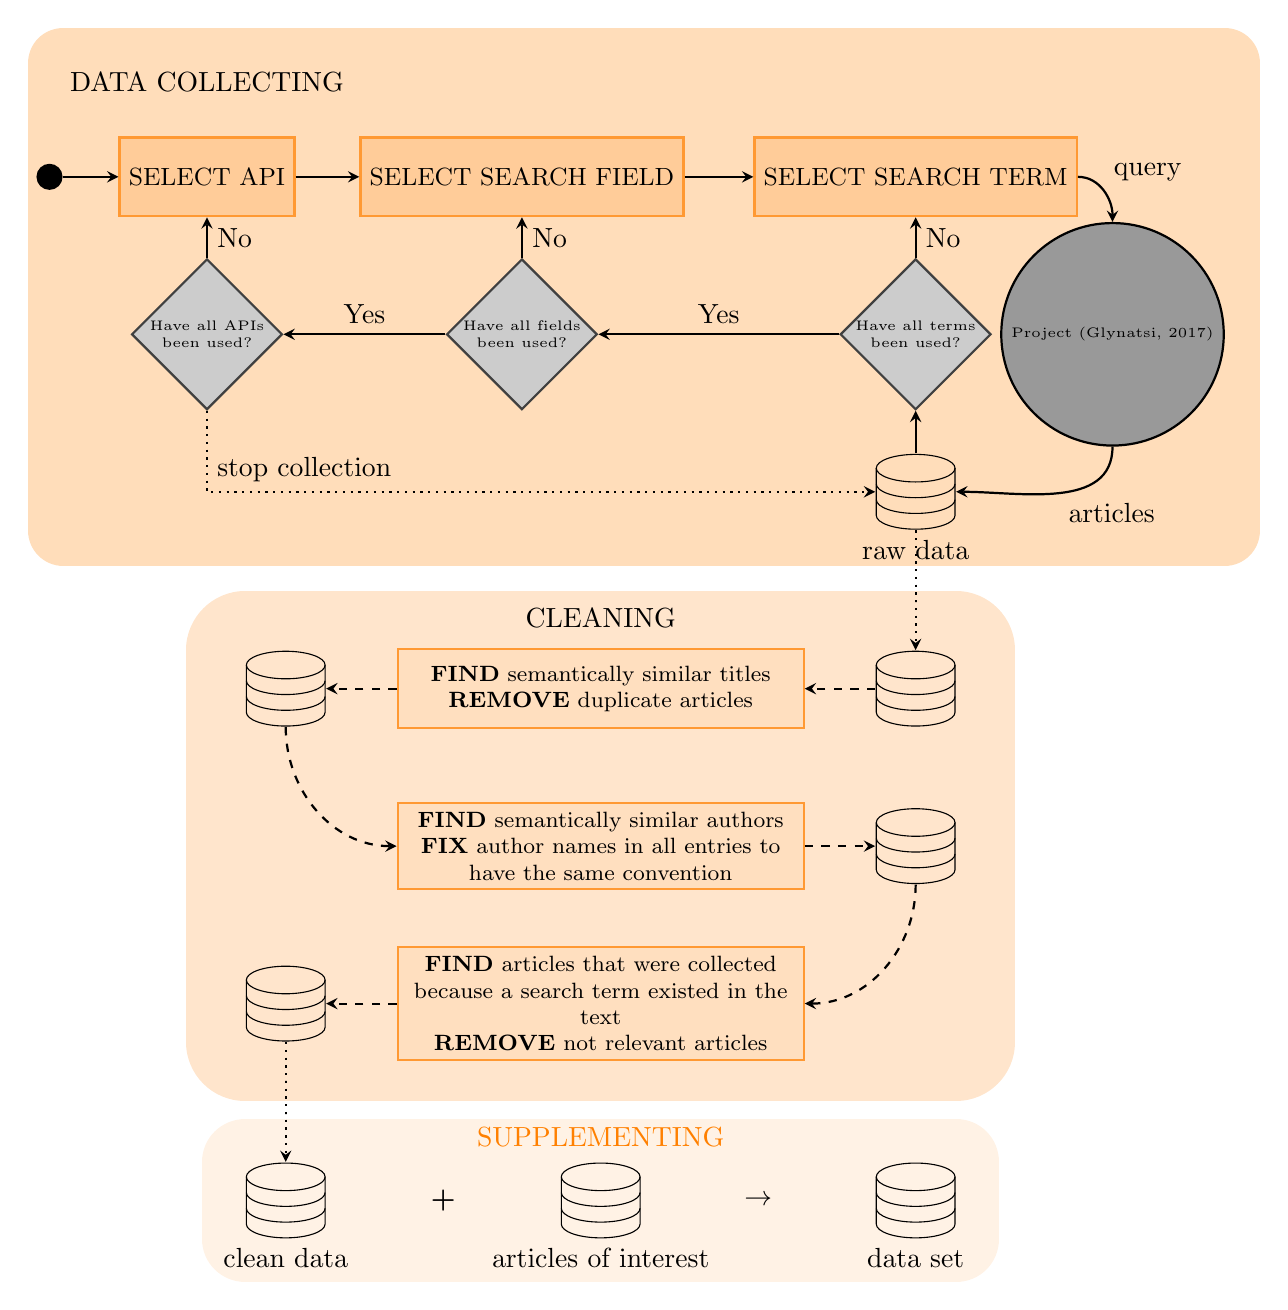
\begin{tikzpicture}[node distance=1.3cm,>=stealth,bend angle=45,auto]

\tikzstyle{place}=[rectangle,thick,draw=orange!80,fill=orange!40, minimum size=10mm,
font=\small]
\tikzstyle{red place}=[circle, thick, draw=black, fill=gray!80, minimum
size=10mm]

\tikzstyle{transition}=[diamond,thick,draw=black!75,
                fill=black!20,minimum size=6mm, font=\tiny, text width=4.5em, text badly centered, node distance=3cm, inner sep=0pt]

\makeatletter
\tikzset{
    database/.style={
        path picture={
            \draw (0, 1.5*\database@segmentheight) circle [x radius=\database@radius,y radius=\database@aspectratio*\database@radius];
            \draw (-\database@radius, 0.5*\database@segmentheight) arc [start angle=180,end angle=360,x radius=\database@radius, y radius=\database@aspectratio*\database@radius];
            \draw (-\database@radius,-0.5*\database@segmentheight) arc [start angle=180,end angle=360,x radius=\database@radius, y radius=\database@aspectratio*\database@radius];
            \draw (-\database@radius,1.5*\database@segmentheight) -- ++(0,-3*\database@segmentheight) arc [start angle=180,end angle=360,x radius=\database@radius, y radius=\database@aspectratio*\database@radius] -- ++(0,3*\database@segmentheight);
        },
        minimum width=2*\database@radius + \pgflinewidth,
        minimum height=3*\database@segmentheight + 2*\database@aspectratio*\database@radius + \pgflinewidth,
    },
    database segment height/.store in=\database@segmentheight,
    database radius/.store in=\database@radius,
    database aspect ratio/.store in=\database@aspectratio,
    database segment height=0.1cm,
    database radius=0.25cm,
    database aspect ratio=0.35,
}
\makeatother

\node (title) at (0, 1.2) {DATA COLLECTING};
\node [circle, black, fill=black] (start) at (-2,0) {};
\node [place] (api) at (0, 0) {SELECT API};
\node [place] (field) at (4, 0) {SELECT SEARCH FIELD};
\node [place] (term) at (9, 0) {SELECT SEARCH TERM};

\node [red place, font=\tiny] (arcas) at (11.5, -2) {Project~(Glynatsi, 2017)};
\node[database,label=below:raw data,database radius=.5cm,database segment
height=0.2cm] (db) at (9,-4) {};

\node [transition] (if_term) at (9, -2) {Have all terms been used?};
\node [transition] (if_field) at (4, -2) {Have all fields been used?};
\node [transition] (if_api) at (0, -2) {Have all APIs been used?};

\begin{pgfonlayer}{background}
    \filldraw [line width=9mm, join=round,orange!27]
      (title.north  -| start.east)  rectangle (db.south  -| arcas.east);
  \end{pgfonlayer}

\draw (start) edge[out=0, in=180, ->, thick] node [] {} (api);
\draw (api) edge[out=0, in=180, ->, thick] node [] {} (field);
\draw (field) edge[out=0, in=180, ->, thick] node [] {} (term);
\draw (term) edge[out=0, in=90, ->, thick] node [] {query} (arcas);
\draw (arcas) edge[out=-90, in=0, ->, thick] node [] {articles} (db);
\draw (db) edge[out=90, in=-90, ->, thick] node [] {} (if_term);


\draw (if_term) edge[out=90, in=-90, ->, thick] node [right] {No} (term);
\draw (if_term) edge[out=180, in=0, ->, thick] node [above] {Yes} (if_field);

\draw (if_field) edge[out=90, in=-90, ->, thick] node [right] {No} (field);
\draw (if_field) edge[out=180, in=0, ->, thick] node [above] {Yes} (if_api);

\draw (if_api) edge[out=90, in=-90, ->, thick] node [right] {No} (api);
\draw[dotted, ->, thick] (if_api) |- node [above right] {stop collection} (db);

% second layer

\node [database,database radius=.5cm,database segment
height=0.2cm] (db_to_clean) at (9, -6.5) {};

\draw (db) edge[out=-90, in=90, ->, thick, dotted] node [above] {} (db_to_clean);

\node [place, draw=orange!80, fill=orange!25, font=\footnotesize, text width=14em, text badly centered] (titles) at (5,
-6.5) {\textbf{FIND} semantically similar titles \textbf{REMOVE} duplicate articles};

\draw (db_to_clean) edge[out=180, in=0, ->, thick, dashed] node  {} (titles);

\node at (5, -5.6) {CLEANING};
\node [database,database radius=.5cm,database segment
height=0.2cm] (db_left) at (1, -6.5) {};

\draw (titles) edge[out=180, in=0, ->, thick, dashed] node  {} (db_left);

\node [place, draw=orange!80, fill=orange!25, font=\footnotesize, text width=14em, text badly centered] (authors) at (5,
-8.5) {\textbf{FIND} semantically similar authors \\ \textbf{FIX} author
names in all entries to have the same convention};

\draw (db_left) edge[out=-90, in=180, ->, thick, dashed] node  {} (authors);

\node [database,database radius=.5cm,database segment
height=0.2cm] (db_right) at (9, -8.5) {};

\draw (authors) edge[out=0, in=180, ->, thick, dashed] node  {} (db_right);

\node [place, draw=orange!80, fill=orange!25, font=\footnotesize, text width=14em, text badly centered] (entries) at (5,
-10.5) {\textbf{FIND} articles that were collected because a search term existed
in the text \\ \textbf{REMOVE} not relevant articles};

\draw (db_right) edge[out=-90, in=0, ->, thick, dashed] node  {} (entries);

\node [database,database radius=.5cm,database segment
height=0.2cm] (db_low) at (1, -10.5) {};

\draw (entries) edge[out=180, in=0, ->, thick, dashed] node  {} (db_low);

\begin{pgfonlayer}{background}
    \filldraw [line width=15mm, join=round,orange!20]
      (db_left.north  -| db_left.west)  rectangle (db_low.south  -| db_right.east);
\end{pgfonlayer}

% last layer

\node[database,label=below:clean data,database radius=.5cm,database segment
height=0.2cm] (db_clean) at (1,-13) {};

\draw (db_low) edge[out=-90, in=90, ->, thick, dotted] node [above] {} (db_clean);

\node at (3, -13) {\textbf{+}};

\node[database,label=below:articles of interest,database radius=.5cm,database segment
height=0.2cm] (db_manual) at (5,-13) {};

\node at (7, -13) {\textbf{$\rightarrow$}};

\node[database,label=below:data set,database radius=.5cm,database segment
height=0.2cm] (db_final) at (9,-13) {};

\begin{pgfonlayer}{background}
    \filldraw [line width=11mm, join=round,orange!10]
      (db_clean.north  -| db_clean.west)  rectangle (db_final.south  -| db_final.east);
\end{pgfonlayer}

\node [orange, ] at (5, -12.2) {SUPPLEMENTING};

\end{tikzpicture}

\end{document}
